\newpage

\section{Congruence Criteria}
In this activity, we show how the common triangle congruence criteria follow from
 what we now know about isometries.\standardhs{G-CO.8}  Recall that two figures are said to be 
congruent if there exists an isometry (translation, rotation, or reflection) or a 
sequence of isometries that maps one figure onto the other.  

\begin{prob}
Proof of Side-Angle-Side (SAS) congruence.  Suppose $\triangle ABC$ and $\triangle XYZ$ are such that $AB=XY$, $AC=XZ$, and $\angle A \cong \angle X$.  Prove, using basic rigid motions, that $\triangle ABC \cong \triangle XYZ$.  Consider the figure below.  
$$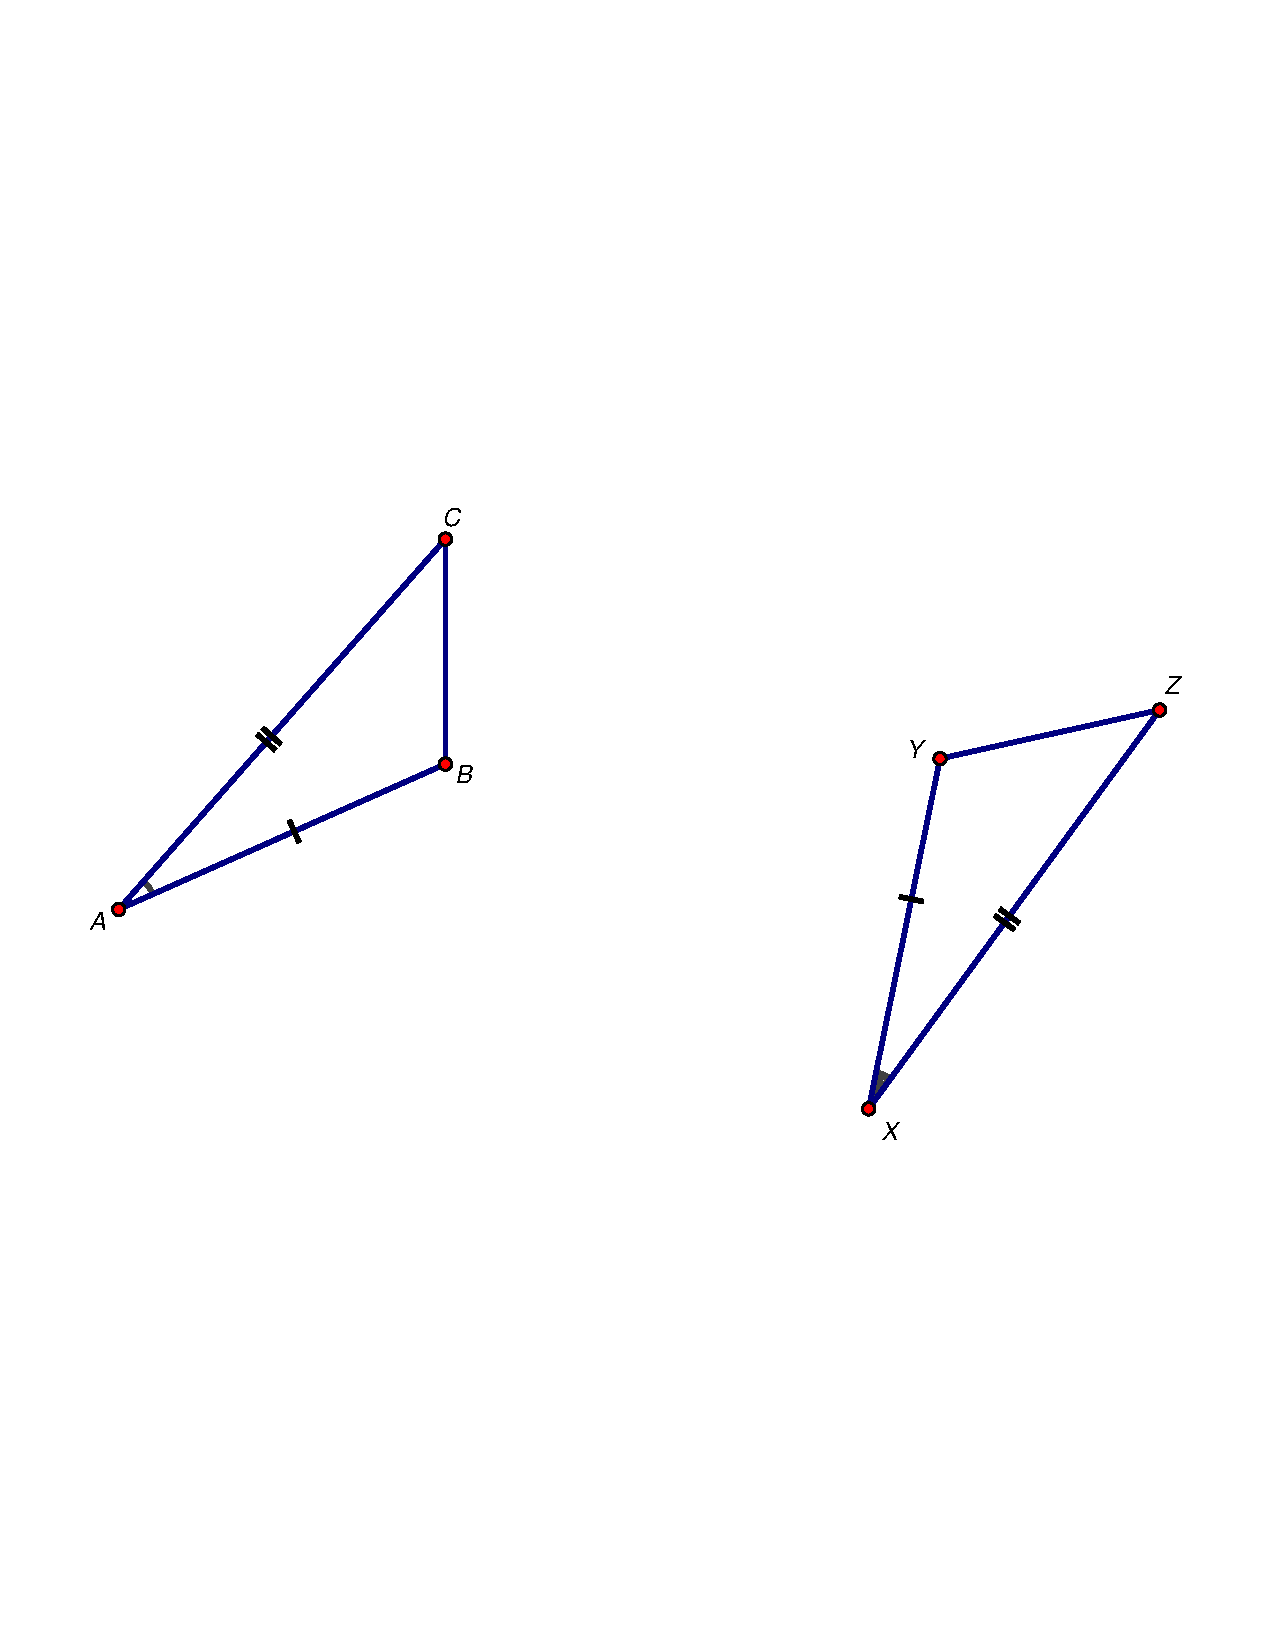
\includegraphics[scale=0.6]{SAS}$$
Fill in the details of the following proof.  
\begin{enumerate}
\item Translate $\triangle ABC$ through the vector $\overrightarrow{AX}$.  Call the image $\triangle A'B'C'$.  Explain why $A'$ and $X$ coincide.
\item Rotate $\triangle A'B'C'$ about $X=A'$ through $\angle B'XY$ so that ray $\overrightarrow{A'B'}$ is along ray $\overrightarrow{XY}$.  Call the image $\triangle A''B''C''$   Explain how you know the segments $\overline{A''B''}$ and $\overline{XY}$ coincide. 
\item Reflect $\triangle A''B''C''$ about the line $\overleftrightarrow{A''B''} = \overleftrightarrow{XY}$.  Call the image $\triangle A'''B'''C'''$.  Explain why $\overline{A'''C'''}$ and $\overline{XZ}$ coincide.
\item Explain how you now know that all sides and angles of $\triangle A'''B'''C'''$ are congruent to the corresponding sides and angles of $\triangle XYZ$.  
\item Explain how to modify the above steps to handle the following different cases: 
\begin{itemize}
\item Initially $X = A$. 
\item After the translation, $\overline{A'B'}$ and $\overline{XY}$ coincide. 
\item After the rotation, $\overline{A''C''}$ and $\overline{XZ}$ coincide.  (Hint:  Consider whether $C''$ and $Z$ are on the same side or on opposite sides of $\overleftrightarrow{XZ}$.)  
\end{itemize}
\end{enumerate}
\end{prob}

\begin{prob}
Proof of Angle-Side-Angle (ASA) congruence.  Suppose $\triangle ABC$ and $\triangle XYZ$ are such that $AB=XY$, $\angle A \cong \angle X$, and $\angle B \cong \angle Y$.  Prove, using basic rigid motions, that $\triangle ABC \cong \triangle XYZ$.  
\begin{enumerate}
\item Outline a general proof for the figure below.  
$$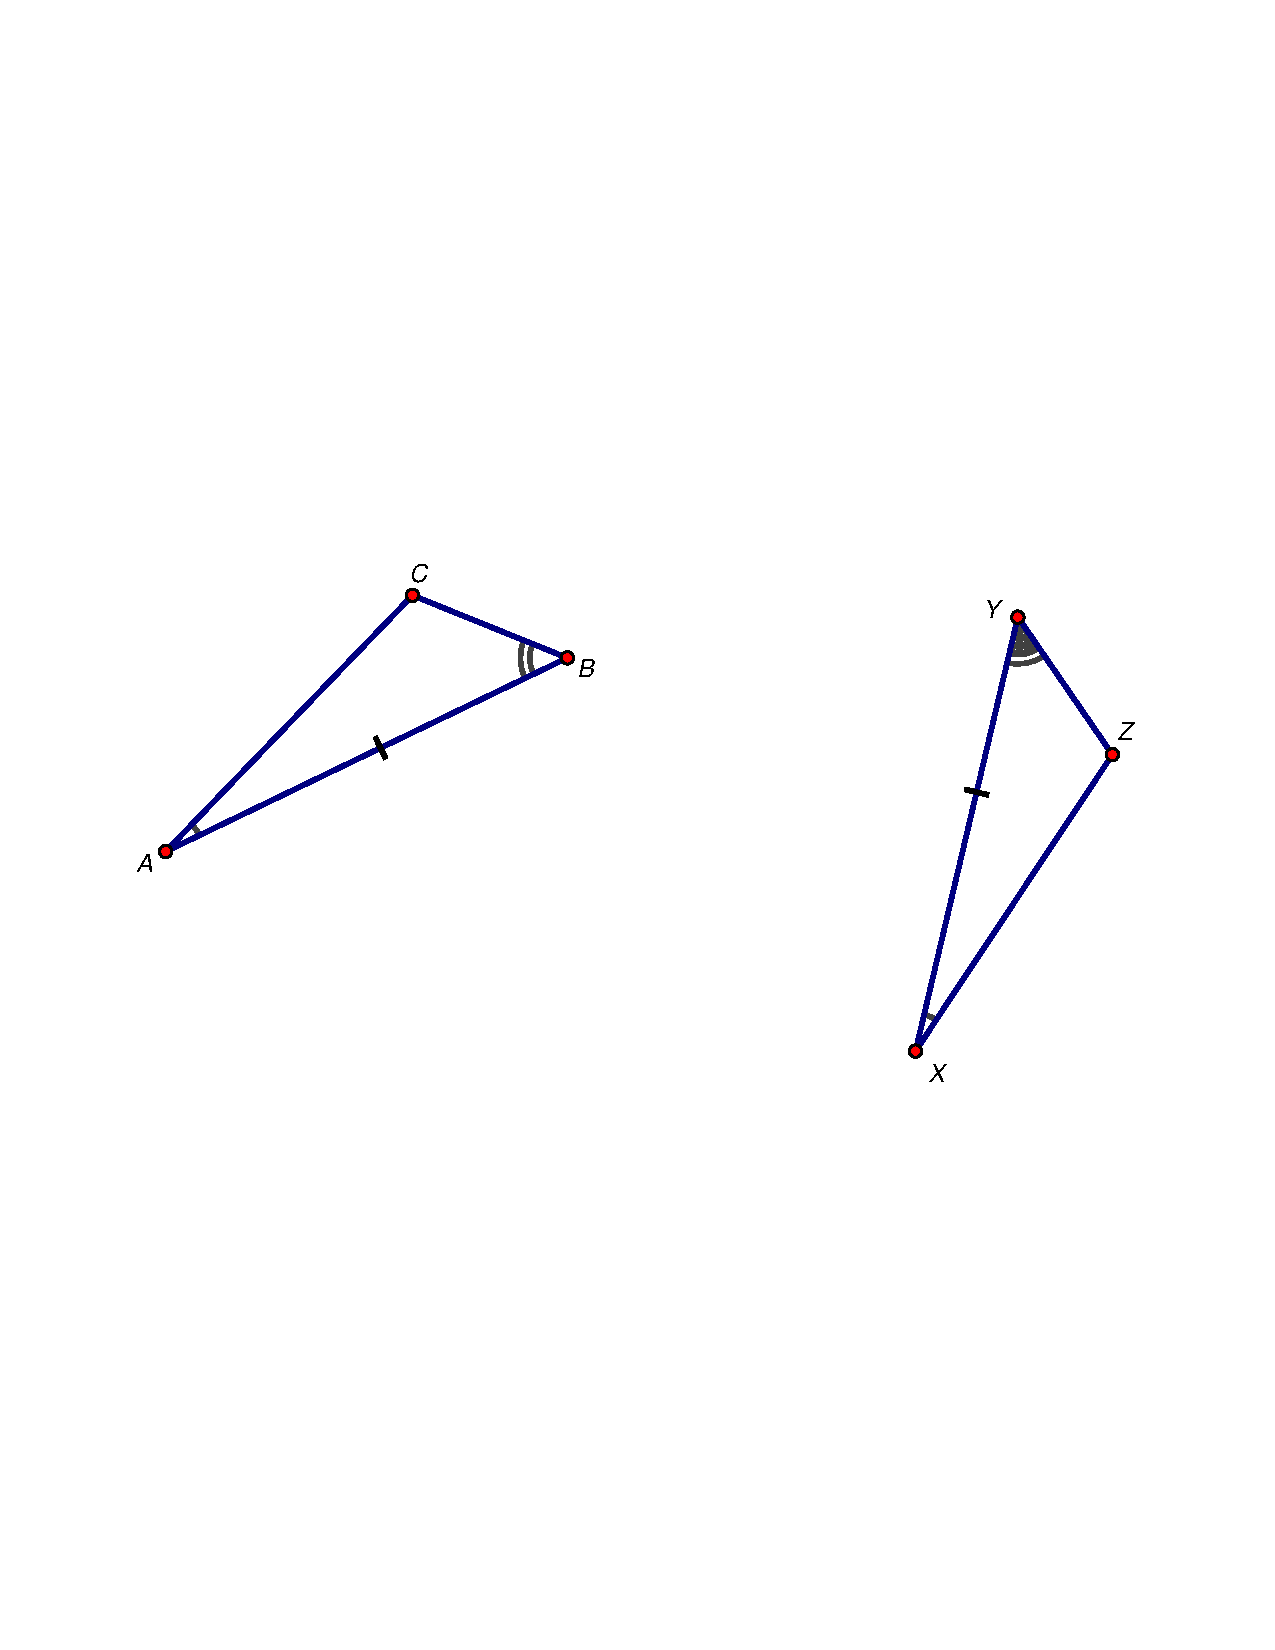
\includegraphics[scale=0.6]{ASA}$$
\item Explain carefully how you know, after the sequence of rigid motions, that the ``final image'' of $C$ coincides with $Z$.  
\item Describe how to modify the outline to handle other cases. 
\end{enumerate}
\end{prob}

\begin{prob}
Proof of Hypotenuse-Leg (HL) congruence.  Suppose $\triangle ABC$ and $\triangle XYZ$ are such that $\angle C$ and $\angle Z$ are right angles, $AB=XY$, and $BC=YZ$.  Prove that $\triangle ABC \cong \triangle XYZ$.  (Hint:  First extend side $\overrightarrow{AC}$ to a point $A'$ so that $CA'=XZ$, and argue that $\triangle A'BC \cong \triangle XYZ$.)  
$$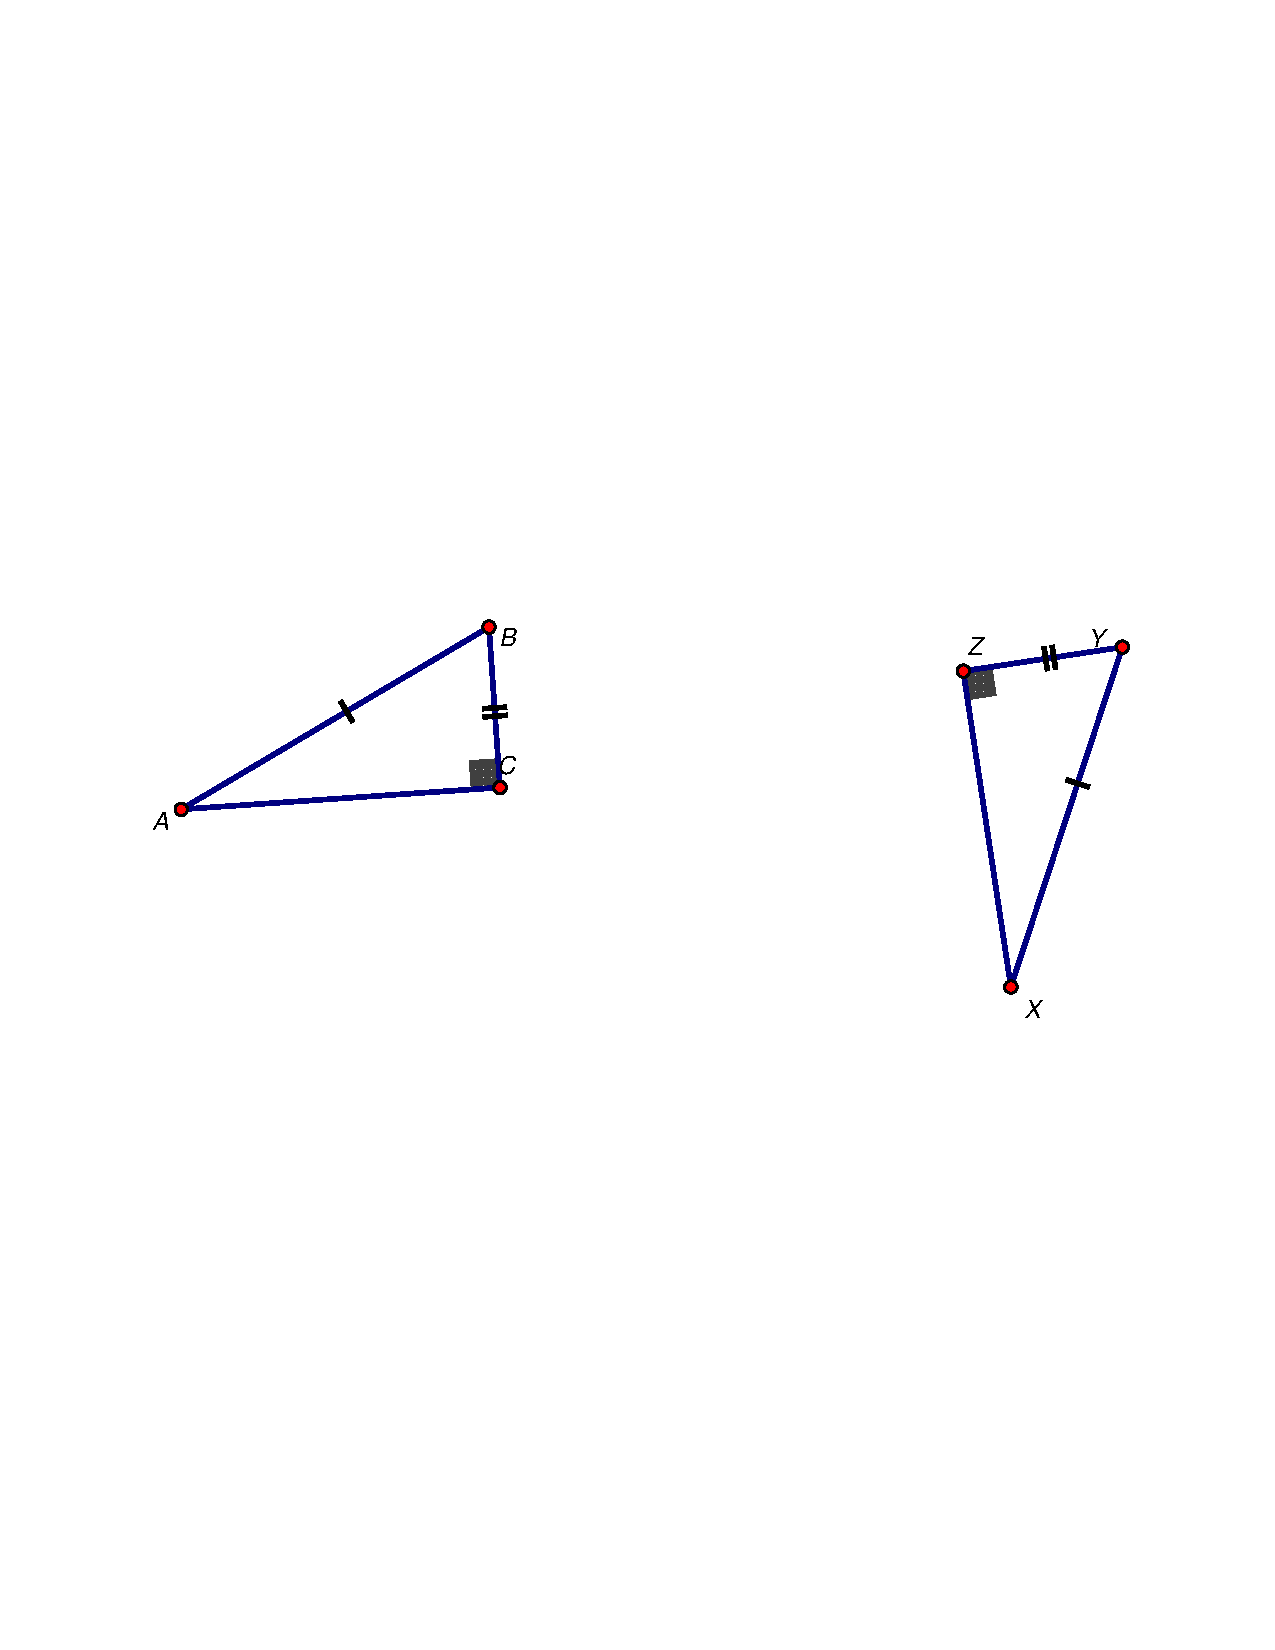
\includegraphics[scale=0.6]{HL}$$
\end{prob}

\begin{prob}
Proof of Side-Side-Side (SSS) congruence.  Suppose $\triangle ABC$ and $\triangle XYZ$ are such that $AB=XY$, $AC=XZ$, and $BC=YZ$.  Prove, using basic rigid motions, that $\triangle ABC \cong \triangle XYZ$.  Build toward the general case through the following steps:  
\begin{enumerate}
\item Case 1a:  $A=X$, $B=Y$, and $C$ and $Z$ lie on opposite sides of $\overleftrightarrow{AB}$.  (Hint:  Explain why the situation must be like one of the figures below, argue that $\overleftrightarrow{AB}$ is the perpendicular bisector of $\overline{CZ}$, and then use a reflection.)
$$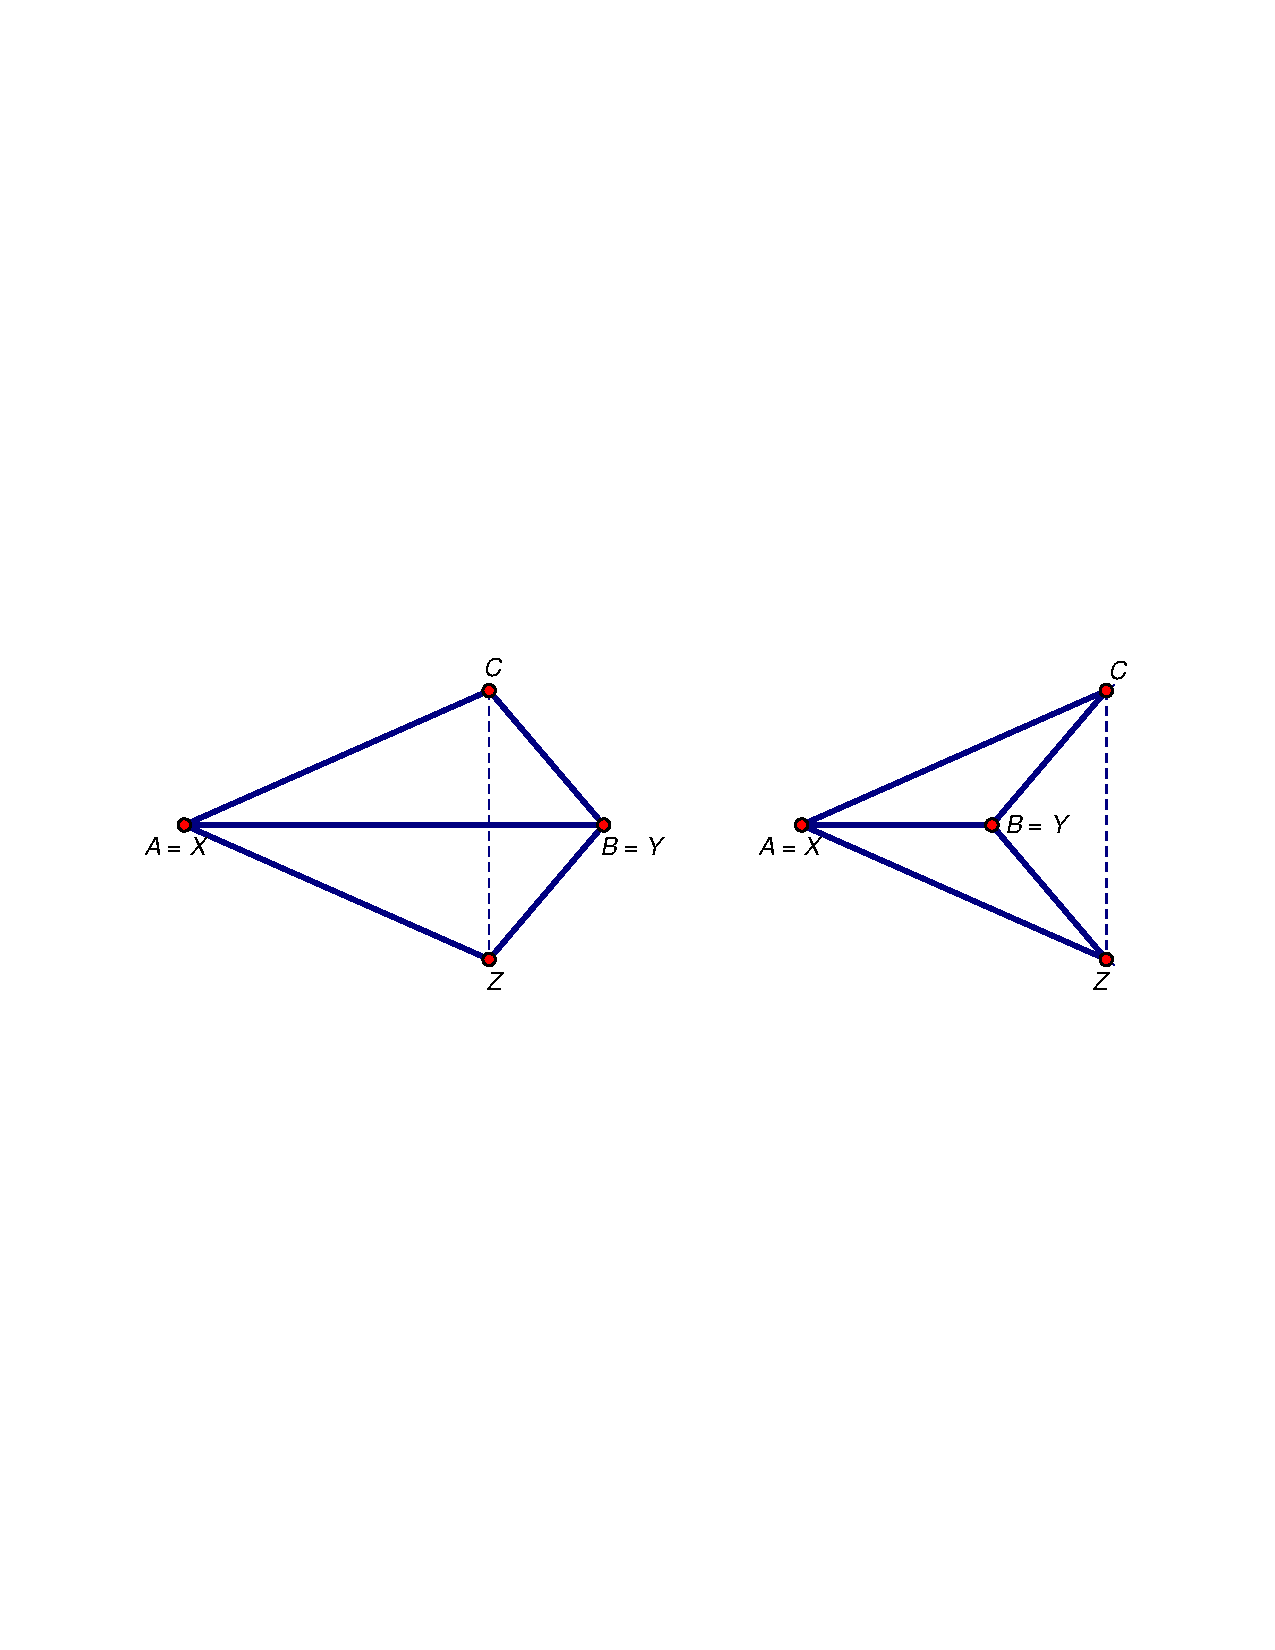
\includegraphics[scale=0.6]{SSS}$$
\item Case 1b:  $A=X$, $B=Y$, and $C$ and $Z$ lie on the same side of $\overleftrightarrow{AB}=\overleftrightarrow{XY}$.  (Hint: Consider a reflection of one of the triangles and use the previous case.)  
\item Case 2:  $A=X$ but $B \ne Y$.
\item Case 3: The general case.  
\end{enumerate}
\end{prob}



